\documentclass{article}
\usepackage{a4wide}
\usepackage{breakurl}             % Not needed if you use pdflatex only.

\usepackage{graphicx,color}
\usepackage{amsmath,amsthm,amscd}
\usepackage{latexsym,amssymb}
\usepackage{enumitem}
\usepackage{tikz}
\usepackage{wrapfig,caption,subcaption}
\usetikzlibrary{matrix,arrows,decorations.pathmorphing}

% %%%%%%%%%%%%%%%%%%%%%

\newtheorem{theorem}{Theorem}[section]
\newtheorem{axiom}{Axiom}%[section]
\newtheorem{proposition}[theorem]{Proposition}%[section]
\newtheorem{lemma}[theorem]{Lemma}%[section]
\newtheorem{corollary}[theorem]{Corollary}%[section]
\newtheorem{hypothesis}[theorem]{Hypothesis}%[section]

\theoremstyle{definition}
\newtheorem{definition}[theorem]{Definition}%[section]
\newtheorem{problem}[theorem]{Problem}%[section]

\newtheorem{example}[theorem]{Example}%[section]
\newtheorem{note}[theorem]{Remark}%[section]
\newtheorem{notation}[theorem]{Notation}%[section]
\newtheorem*{axioms}{Axioms}
\newtheorem*{syntax}{Syntax}
\newtheorem*{semantics}{Semantics}

\newcommand{\defn}[1]{Definition~\ref{defn:#1}}
\newcommand{\fig}[2][]{Figure~\ref{fig:#2}\ensuremath{#1}}
\newcommand{\tab}[1]{Table~\ref{tab:#1}}
\newcommand{\eq}[1]{(\ref{eq:#1})}
\newcommand{\res}[1]{(\ref{res:#1})}
\newcommand{\ex}[1]{Example~\ref{ex:#1}}
\newcommand{\secn}[1]{Section~\ref{sec:#1}}
\newcommand{\rem}[1]{Remark~\ref{rem:#1}}
\newcommand{\lem}[1]{Lemma~\ref{lem:#1}}
\newcommand{\cor}[1]{Corollary~\ref{cor:#1}}
\newcommand{\thm}[1]{Theorem~\ref{thm:#1}}
\newcommand{\app}[1]{Appendix~\ref{app:#1}}
\newcommand{\axs}[1]{Axioms~\ref{ax:#1}}
\newcommand{\axss}[2]{Axioms~\ref{ax:#1}, \ref{ax:#2}}
\newcommand{\ax}[1]{Axiom~\ref{ax:#1}}
\newcommand{\prop}[1]{Proposition~\ref{prop:#1}}

\newcommand{\mycaption}[1]{\caption{#1.}}

% %%%%%%%%%%%%%%%%%%%%%

\newcommand{\mdash}[1][]{---#1}
\newcommand{\ndash}[1][]{--#1}
\newcommand{\ie}[1][\ ]{i.e.{#1}}
\newcommand{\eg}{e.g.\ }
\newcommand{\cf}{cf.\ }
%% \newcommand{\nb}[1]{\marginpar{\emph{N\!\!B}:\ #1}}
\newcommand{\nb}[1]{\marginpar{/#1/}}

\newcommand{\bydef}[1]{\ensuremath{\stackrel{\Delta}{#1}}}
\newcommand{\oftype}{\ensuremath{\!:\!}}
\newcommand{\suchthat}{\ensuremath{\,|\,}}
\newcommand{\rightsuchthat}{\ensuremath{\,\right|\,}}
\newcommand{\leftsuchthat}{\ensuremath{\,\left|\,}}
\newcommand{\setdef}[2]{\ensuremath{\{{#1}\,|\,{#2}\}}}
\newcommand{\Setdef}[2]{\ensuremath{\Big\{{#1}\,\Big|\,{#2}\Big\}}}
\newcommand{\fire}[1]{\ensuremath{\dot{#1}}}
\newcommand{\act}[1]{\ensuremath{#1}}
\newcommand{\inhib}[1]{\ensuremath{\overline{#1}}}
\newcommand{\non}[1]{\ensuremath{\overline{#1}}}
\newcommand{\firesup}[1]{\ensuremath{\mathbf{fire}{\left(#1\right)}}}
\newcommand{\actsup}[1]{\ensuremath{\mathbf{act}{\left(#1\right)}}}
\newcommand{\negsup}[1]{\ensuremath{\mathbf{neg}{\left(#1\right)}}}
\newcommand{\offer}[1][]{\ensuremath{\!\uparrow\!{#1}}}
\newcommand{\noffer}[1][]{\ensuremath{\!\not\,\uparrow\!{#1}}}
\newcommand{\goesto}[1][]{\ensuremath{\stackrel{#1}{\rightarrow}^{}}}
\newcommand{\longgoesto}[1][]{\ensuremath{\stackrel{#1}{\longrightarrow}}}
\newcommand{\symmdiff}[2]{\ensuremath{{#1}\triangle{#2}}}
\newcommand{\glue}[1][]{\ensuremath{{\cal G}^{#1}}}
\newcommand{\glues}{\ensuremath{{\cal G}lue}}
\newcommand{\less}{\prec}

\newcommand{\pin}{\ensuremath{P^{g}}}
\newcommand{\pout}{\ensuremath{P^{r}}}

\newcommand{\true}{\ensuremath{\mathtt{tt}}}
\newcommand{\false}{\ensuremath{\mathtt{ff}}}

\newcommand{\intsem}[1]{\ensuremath{\|{#1}\|}}
\newcommand{\aisem}[1]{\ensuremath{|{#1}|}}

\newcommand{\ai}{\ensuremath{\mathcal{A\hspace{-0.6ex}I\!}}}
\newcommand{\ct}{\ensuremath{\mathcal{T\!}}}
\newcommand{\cru}{\ensuremath{\mathcal{CR\!}}}
\newcommand{\ac}{\ensuremath{\mathcal{AC}\!}}

\newcommand{\cA}{\ensuremath{\mathcal{A}}}
\newcommand{\sB}{\ensuremath{\mathbb{B}}}
\newcommand{\bB}{\ensuremath{\mathbf{B}}}
\newcommand{\cB}{\ensuremath{\mathcal{B}}}
\newcommand{\cC}{\ensuremath{\mathcal{C}}}
\newcommand{\cD}{\ensuremath{\mathcal{D}}}
\newcommand{\sC}{\ensuremath{\mathbb{C}}}
\newcommand{\sE}{\ensuremath{\mathbb{E}}}
\newcommand{\cF}{\ensuremath{\mathcal{F}}}
\newcommand{\cG}{\ensuremath{\mathcal{G}}}
\newcommand{\cH}{\ensuremath{\mathcal{H}}}
\newcommand{\cI}{\ensuremath{\mathcal{I}}}
\newcommand{\sI}{\ensuremath{\mathbb{I}}}
\newcommand{\cM}{\ensuremath{\mathcal{M}}}
\newcommand{\cN}{\ensuremath{\mathcal{N}}}
\newcommand{\sN}{\ensuremath{\mathbb{N}}}
\newcommand{\cP}{\ensuremath{\mathcal{P}}}
\newcommand{\sP}{\ensuremath{\mathbb{P}}}
\newcommand{\cQ}{\ensuremath{\mathcal{Q}}}
\newcommand{\sQ}{\ensuremath{\mathbb{Q}}}
\newcommand{\cR}{\ensuremath{\mathcal{R}}}
\newcommand{\sR}{\ensuremath{\mathbb{R}}}
\newcommand{\cS}{\ensuremath{\mathcal{S}}}
\newcommand{\sS}{\ensuremath{\mathfrak{S}}}
\newcommand{\cT}{\ensuremath{\mathcal{T}}}
\newcommand{\sT}{\ensuremath{\mathbb{T}}}
\newcommand{\sZ}{\ensuremath{\mathbb{Z}}}

\newcommand{\derrule}[3][1]{%
  \ensuremath{%
    \begin{array}{*{#1}{@{\hspace{2mm}}c@{\hspace{2mm}}}}
      #2\\
      \hline
      \multicolumn{#1}{c}{#3}
    \end{array}%
  }%
}

\newlength{\algowidth}
\setlength{\algowidth}{\textwidth}
\addtolength{\algowidth}{-40pt}

\title{Conversations in BIP: Externalised and Internalised Approaches}

\author{Simon Bliudze
\thanks{EPFL, Rigorous System Design Laboratory, Station 14, 1015 Lausanne,
Switzerland; firstname.lastname@epfl.ch}
\and Marius Bozga
\thanks{Verimag}
\and Mohamad Jaber
\thanks{American University of Beirut} 
\and Joseph Sifakis
\footnotemark[1]
}

\date{}

\begin{document}

\maketitle

\begin{abstract}
\end{abstract}

% *********************************************************************
% *********************************************************************

\section{Introduction}
\label{sec:intro}


% *********************************************************************
% *********************************************************************

\section{Formal Model}
\label{sec:formal}

% *********************************************************************

\subsection{Grant-Request Labelled Transition Systems}
\label{sec:model}

Intuitively, we consider systems built from a number of components, each
modelled by a labelled transition system (LTS).  In order to perform a
transition, a basic component, which we call {\em behaviour}, issues a
number of requests, which are defined by the transition label and can be
granted by higher-level components, which we call {\em conversations}.
Thus, in general, a complete transition label consists of two sets of {\em
  ports}, representing requests the transition must grant and those it must
obtain in order to be executed.  Below we present a formal model specifying
such behaviour as well as the implied composition operator.

\begin{definition}[\compmodel{} and interactions]
\label{defn:lts}
A \emph{Grant-Request Labelled Transition System} (\compmodel{}) is a
quadruple $(Q,\pin,\pout,\goesto[])$, where $Q$ is a finite set of states,
$\pin \cap \pout = \emptyset$ are finite sets of respectively {\em grant}
and {\em request} ports and $\goesto[] \subseteq Q \times 2^P \times Q$
(with $P = \pin \cup \pout$) is a transition relation.  Transitions are
labelled by \emph{interactions} $\emptyset \neq a \subseteq P$.  We define
$q \goesto[a] q' \bydef{=}\Big((q, a, q') \in \goesto[]\Big)$ and $q
\goesto[a]\, \bydef{=}\Big(\exists q' \in Q: q \goesto[a] q'\Big)$.
\end{definition}

\begin{notation}
  \label{ntn:lts}
  In \defn{lts} and below, we skip the index on $\goesto_i$ since it is
  always clear from the context.  For a \compmodel{} with the sets of grant
  and request ports respectively $\grant{X}$ and $\request{X}$ (here, $X$
  can be $P$, $P_i$, \etc[]) we will always denote $X \bydef{=} \grant{X}
  \cup \request{X}$.
\end{notation}

\begin{definition}[System]
  \label{defn:system}
  Let $S = \setdef{T_i = (Q_i, \pin_i, \pout_i, \goesto)}{i \in [1,n]}$ be
  a finite set of \compmodel{} and denote $\pin \bydef{=} \bigcup_{i=1}^n
  \pin_i$ and $\pout \bydef{=} \bigcup_{i=1}^n \pout_i$.  $S$ is a {\em
    system} iff the following two conditions hold:
  \begin{enumerate}
  \item the sets of request ports of all the {\em components} are pairwise
    disjoint, \ie $\forall i \neq j,\ \pout_i \cap \pout_j = \emptyset$;
  \item any grant port belonging to more than one component is also a
    request port of some component, \ie $\forall p, \left(\exists i \neq 
    j: p \in \pin_i \cap \pin_j \implies p \in \pout\right)$.
  \end{enumerate}

  A system is {\em closed} if $\pin \subseteq \pout$.  Otherwise it is {\em
    open}.
\end{definition}

To simplify the presentation, below we postulate that for any $q$, the
predicate $q \goesto[\emptyset] q$ is true, whenever it appears in the
premises of an SOS rule.

\begin{definition}[Operational semantics of a system]
  \label{defn:composition}
  The operational semantics of a system $S = \Setdef{T_i = (Q_i, \pin_i,
  \pout_i, \goesto)}{i \in [1,n]}$ is given by a \compmodel{} $\compose[S]
  \bydef{=} (Q, \pin, \pout, \goesto)$, where
  \begin{equation}
    \label{eq:composition:ports}
    Q = \prod_{i=1}^n Q_i\,,
    \hspace{1cm}
    \pin = \bigcup_{i=1}^n \pin_i \setminus \bigcup_{i=1}^n \pout_i\,,
    \hspace{1cm}
    \pout = \bigcup_{i=1}^n \pout_i \setminus \bigcup_{i=1}^n \pin_i 
  \end{equation}
  and $\goesto$ is the minimal transition relation inductively defined by
  the derivation rule
  \begin{equation}
    \label{eq:composition:transitions}
    \renewcommand{\arraystretch}{1.5}
    \derrule[3]{
      a \subseteq \bigcup_{i=1}^n P_i &
      \forall i \in [1,n],\, (a \cap P_i \neq \emptyset \implies 
        q_i \longgoesto[a \cap P_i] q_i') &
      \forall i \in [1,n],\, (a \cap P_i = \emptyset \implies q_i = q_i') 
    }{
      q_1 \dots q_n \longgoesto[a \cap P] q_1' \dots q_n'
    }\,,
  \end{equation}
  with $P_i$ and $P$ as in \ntn{lts}.
\end{definition}

\begin{proposition}
  \label{prop:associativity}
  Composition operator $\compose$ in \defn{composition} is associative.
\end{proposition}

\begin{definition}[Behaviour and conversation]
  \label{defn:components}
  A \compmodel{} $(Q, \pin, \pout, \goesto)$ is
  \begin{itemize}
  \item a {\em behaviour} if $\pin  = \emptyset$;
  \item a \emph{conversation} if, for any transition $q \goesto[a] q'$, both
    $a \cap \pin \neq \emptyset$ and $a \cap \pout \neq \emptyset$.
  \end{itemize}
\end{definition}

Conversations represent sequences of interactions. They are used to compose
behaviours.  Notice that operational semantics of a closed system is a
behaviour.  Below we will only consider systems, whereof each component is
either a behaviour or a conversation.

\begin{example}[BIP interaction models]
  \label{ex:bip}
  Let $B_i = (Q_i, \emptyset, \pout_i, \goesto)$, for $i \in [1,n]$, be a
  set of behaviours with pairwise disjoint ports.  Consider $P =
  \bigcup_{i=1}^n \pout_i$ and let $\gamma \subseteq 2^P$ be a BIP
  interaction model \cite{BliSif07-acp-emsoft}.  The conversation $C_\gamma
  = \Big(\{*\}, P, \gamma, \Setdef{* \longgoesto[a\cup\{a\}] *}{a \in
  \gamma}\Big)$ realises the same coordination as the one imposed by
  $\gamma$, \ie $C_\gamma(B_1, \dots, B_n) \bydef{=} \compose[\{C_\gamma,
  B_1, \dots, B_n\}] = \gamma(B_1, \dots, B_n)$, where the latter is the
  composed component obtained by applying the interaction model $\gamma$ to
  behaviours $B_1, \dots, B_n$ with the operational semantics defined in
  \cite{BliSif07-acp-emsoft}.
\end{example}

\begin{example}[Network sort]
  \label{ex:network}
  ...
\end{example}

\begin{definition}[Topologies]
  The {\em topology} of a system $S$ is a directed graph $\topo{S} =
  (S, E)$, having the components of the system as vertices and the set
  of edges $E = \setdef{(T_i,T_j)}{\pout_i \cap \pin_j \neq
    \emptyset}$.  In other words, there is an edge from $T_i$ to $T_j$
  if some of the requests of the former can be granted by the latter.

  If $\topo{S}$ is a directed acyclic graph (DAG), the $S$ is a {\em
  flow-system}.  If $\topo{S}$ is disconnected, \ie $E = \emptyset$, the
  system is {\em independent}.
\end{definition}

Observe that any non-trivial (\ie non-empty) closed flow-system $S$
necessarily contains a certain number of behaviours.  Each conversation can
be assigned a {\em level} defined as the maximal length of a directed path
in $\topo{S}$ from some behaviour to this conversation.

Composition defined by the operational semantics of systems allows
simultaneous execution of interactions authorised by any number of
top-level conversations.  However, mutual exclusion can be ensured by
applying a single top-level arbiter conversation.  Such arbiter
conversation can enforce simple non-deterministic mutual exclusion, as in
\ex{bip}, or any complex scheduling protocol, \eg Round-Robin.

% *********************************************************************

\subsection{Data Management and Transfer in Flow-Systems}
\label{sec:data}

We now extend the definitions of \secn{model} to incorporate data.  To
avoid dealing with causality cycles, we limit ourselves to flow-systems,
where causal data dependencies can be unambigously resolved.  Intuitively,
in each cycle, we propagate the data from behaviours upwards through all
relevant conversations.  At each component, this data can influence the
decision as to what transitions are enabled.  Finally, once a global
interaction has been choosen at the top level, the updated data is
propagated back to behaviours.  Below, we present this in a formal manner.

\begin{definition}[\compmodel{} with data]
  A {\em \compmodel{} with data} is a tuple $(T, \data[i], \data[l],
  \data[o], up, down)$, where $T = (Q, \pin, \pout, \goesto)$ is a
  \compmodel{}, $\data[i]$, $\data[l]$ and $\data[o]$ are respectively the
  domains of {\em input}, {\em local} and {\em output} data, and $up$ and
  $down$ are mappings from the transition relation $\goesto$ to
  functions $(\data[l] \times \data[o])^{\data[i]}$ and $\data$
\end{definition}
% *********************************************************************

\subsection{Expressiveness Results}
\label{sec:expressiveness}


Types of conversations:
\begin{itemize}
\item Linear (finite or cyclic) vs.\ branching.  Branching can be
  \begin{itemize}
  \item deterministic
  \item non-deterministic
  \end{itemize}
\item With or without memory (``unbounded'' data values)
\item One label vs.\ multiple ``send'' labels for interactions composing
  the conversation
\end{itemize}

Conversations (deterministic or not) are strictly more expressive than
interactions.

Deterministic and non-deterministic conversations without memory are
equivalent.

Non-deterministic conversations with memory are strictly more expressive
than deterministic conversations with memory

\section{Java Implementation}
\label{sec:java}
We have implemented in Java a model consisting of a set of classes that represents {\compmodel} model. We distinguish mainly between two abstract classes \texttt{Behavior} and \texttt{Conversation}. You define a new behavior as follows:
\begin{itemize}
\item Create a new class that extends \texttt{Behavior} class. 
\item Create instance variables that represent locations, data variables and send/request ports assigned with data variables.
\item Create a constructor method that sets the initial location and create the set of transitions representing the behavior. 
\item Each transition consists of the source location, target location, guard, send/request port, and action. By default, the guard is \texttt{true} and the action is empty.  
\end{itemize}
In the same way, we define a new conversation except that (1) it extends \texttt{Conversation} class; (2) it may contain receive/grant ports; (3) its transitions consist of a source location, target location, set of receive/grant ports, guard, upward action, send/request port, and downward action.

Finally, we create a class that extends \texttt{Compound} class representing the system. In that class, we instantiate behaviors and conversations and we connect receive/grant ports to their corresponding send/request ports. 


We have implemented the semantic proposed in Section \ref{sec:formal}. More precisely, we create a Java thread per behavior instance and another thread that plays as arbiter for selecting a top conversation component to be executed and down propagated. The execution flow is done as follows. Behaviors evaluate the guards of the their current outgoing transitions and notify the corresponding send ports accordingly. A send/request port notifies all of its corresponding receive/grant ports. When a receive/grant port, of a conversation component, has been notified, we identify the set of the current outgoing transitions where all their receive ports have been notified. We evaluate the guards of those transitions and we execute the corresponding upward action when the guard is evaluated to true. Note that, the upward action does not modify the actual data of a conversation component but it creates a copy of its data. This is due to the fact that conversation components could be non-deterministic. That is, more than one of the current outgoing transitions of a given conversation component could be enabled. Each of which has an upward action that may modify the data of that component. For this, components' variables should be of type \texttt{WrapType}. \texttt{WrapType} contains the actual value of a variable and a map from indices to values. It also contains \texttt{getVal} and \texttt{setVal()} methods. 
For a given index, \texttt{getVal()} returns the actual value if the index does not exist in the map, otherwise it returns the corresponding value using the map. \texttt{setVal()} adds the given index along with the given value to the map. 

If the transition has a send/request port, we notify that port with an index. That is, an index identifies a transition and it also identifies the indices of the corresponding receive ports of that transition. 
Note that, a receive port has a direct access to the variables of its corresponding send port. Recall that, the guard of a given transition depends on the value of the variables attached to the send ports that are connected to the receive ports of that transition. So that, before evaluating the guard of a given transition of conversation component, we need first to set the corresponding indices of the bottom conversation components so that \texttt{getVal()} will return the right value. Note that, the upward notifications are done by behaviors' components, that is are done in parallel. For this, before setting the indices of the bottom components, we need first to lock those components to avoid the evaluation of other guards that depend on those components but with different indices. 

Moreover, before executing the upward action we increment the index that represents the current evaluated transition, so that \texttt{setVal()} sets the values properly. 


When all receive ports have been notified, the arbiter thread will be fired. Now, behaviors' components are waiting.  The arbiter selects a top enabled transition of a conversation component (i.e., a transition without a send port, or with a send port but not connected). If such a transition does not exist, the system is deadlocked. Otherwise, the arbiter sets the indices of the bottom components of the selected transition and it executes the down action. Then, it updates the original values w.r.t the index of the selected transition. After that, it recursively notifies the corresponding send port connected to the receive ports of that transition. If a send port belongs to a behavior's component, we disable recursively all other send ports that belong to that component. Then, We check for another top enabled transition of another conversation component. If there is no top enabled transition, the arbiter notifies behavior's components to execute the action of the notified send ports. 


The complexity of this propagation is due to the non-determinism of conversation components. Also, locking bottom components drastically reduces the efficiency of the implementation. As most of the systems consist of conversation components that are deterministic. That is, from any location, at maximum one of the outgoing transitions could be enabled. This can be satisfied if for all locations (1) there exist at maximum one outgoing transition; or (2) the guards of all outgoing transitions are mutually exclusive. In that case, the indices are useless as well as locking of bottom conversation components.
For this, we have developed two implementations that assume non-deterministic and deterministic conversation components, respectively. Clearly, non-determinism of conversation components adds more expressiveness but introduces some overhead. 




\begin{figure}
\centering
\begin{subfigure}[b]{0.71\textwidth}
\centering
\begin{lstlisting}[style=customJava]
public class Generator extends Behavior {
  private Location l0 = new Location(this);
  public SendPort s = new SendPort(this);
  public Generator(Compound compound) {
    super(compound);
    setInitial(l0);
    addTransition(new Transition(l0,l0,s) {
      // default guard and action
    });
  }
}

public class Modulo2 extends Conversation {
  private Location l0 = new Location(this);
  private Location l1 = new Location(this); 
  public SendPort s = new SendPort(this);
  public ReceivePort r = new ReceivePort(this);
		
  public Modulo2(Compound compound) {
    super(compound);
    setInitial(l0);
    addTransition(new TransitionConversation(l0, l1, null, r) { });
    addTransition(new TransitionConversation(l1, l0, s, r) { });
  }
}

public class Modulo8  extends Compound {
  public Modulo8() {
    // Behavior Component
    Generator g = new Generator(this);
		
    // Conversation Components
    Modulo2 R0 = new Modulo2(this, "R0");
    Modulo2 R1 = new Modulo2(this, "R1");
    Modulo2 R2 = new Modulo2(this, "R2");
		
    // Connections
    R0.r.connect(g.s);
    R1.r.connect(R0.s);
    R2.r.connect(R1.s);
  }
}
\end{lstlisting}
\end{subfigure}%
\quad
\begin{subfigure}[b]{0.25\textwidth}
\centering
\scalebox{0.75}{\input{fig/modulo8.pdf_t}}
\end{subfigure}
\caption{Modulo-8 Counter in \compmodel}\label{fig:modulo8}
\end{figure}

Figure \ref{fig:modulo8} shows an example of Modulo-8 counter modeled using {\compmodel} model. 

\subsection{Network Sorting Algorithm}
\label{subsec:nsa}
We consider $2^n$ behaviors, each containing an array of $N$ items. The goal is to sort the items, so that all the items in the first component are smaller than those of the second component and so on. Figure \ref{fig:nsa1} shows a {\compmodel} of the Network Sorting Algorithm for $n=3$.
\begin{figure}
\centering
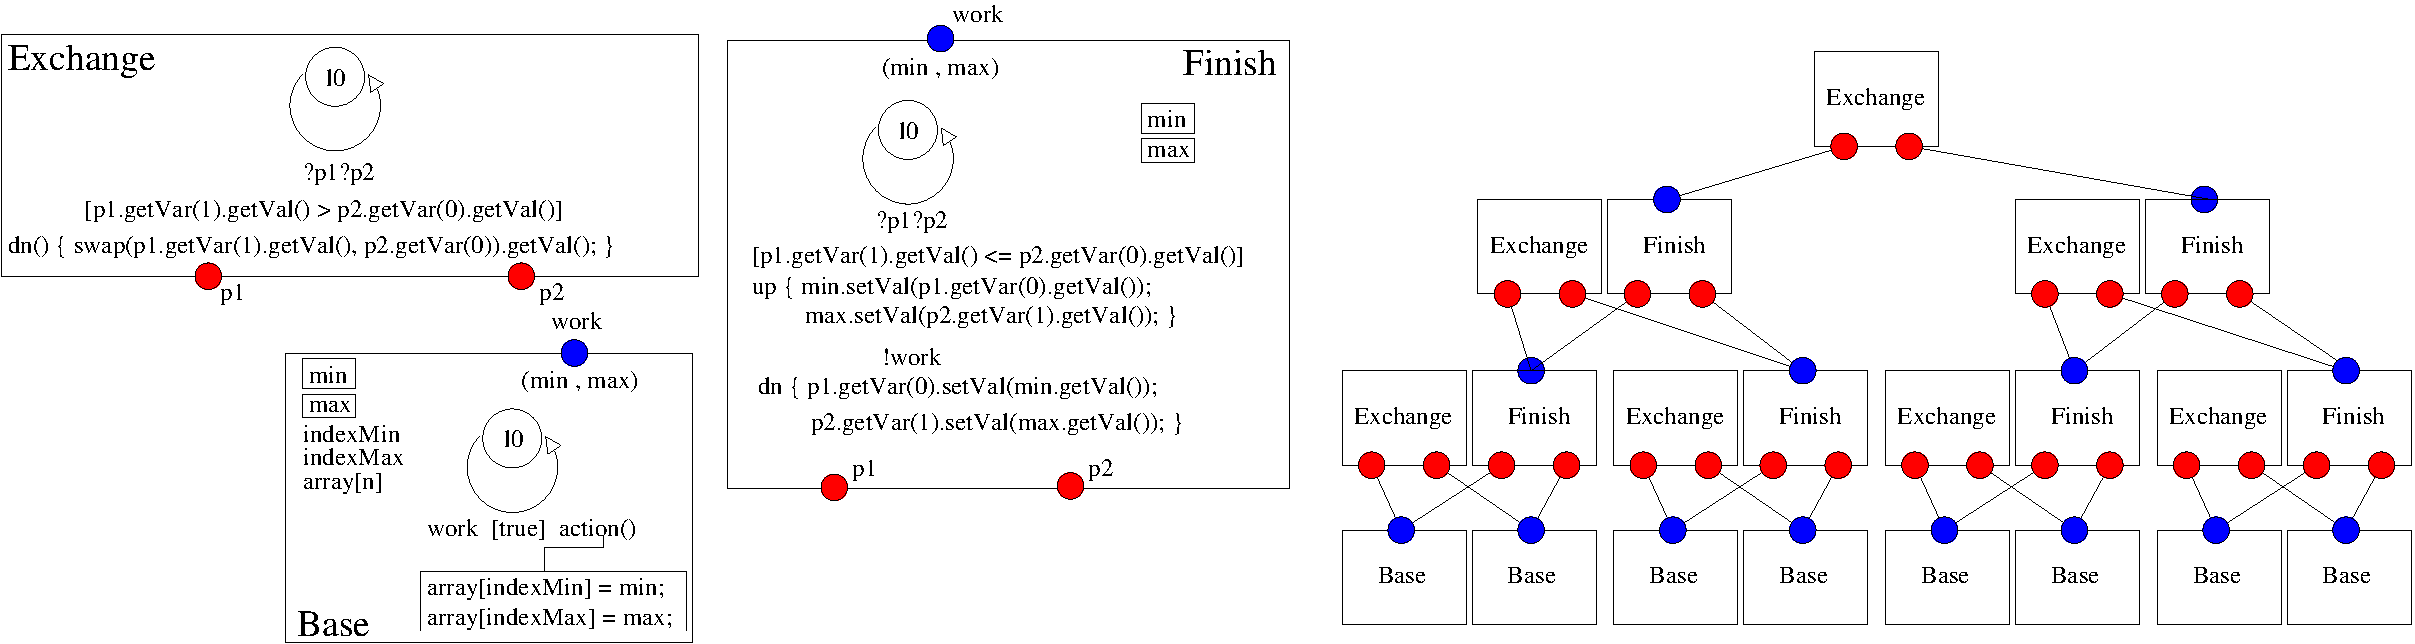
\includegraphics[scale=0.4]{fig/nsav1.pdf}
\caption{Network Sorting Algorithm in {\compmodel}}\label{fig:nsa1}
\end{figure} 
We have also modeled another (see Fig. \ref{fig:nsa2}) version where we merge the Exchange and Finish behaviors. 

\begin{figure}
\centering
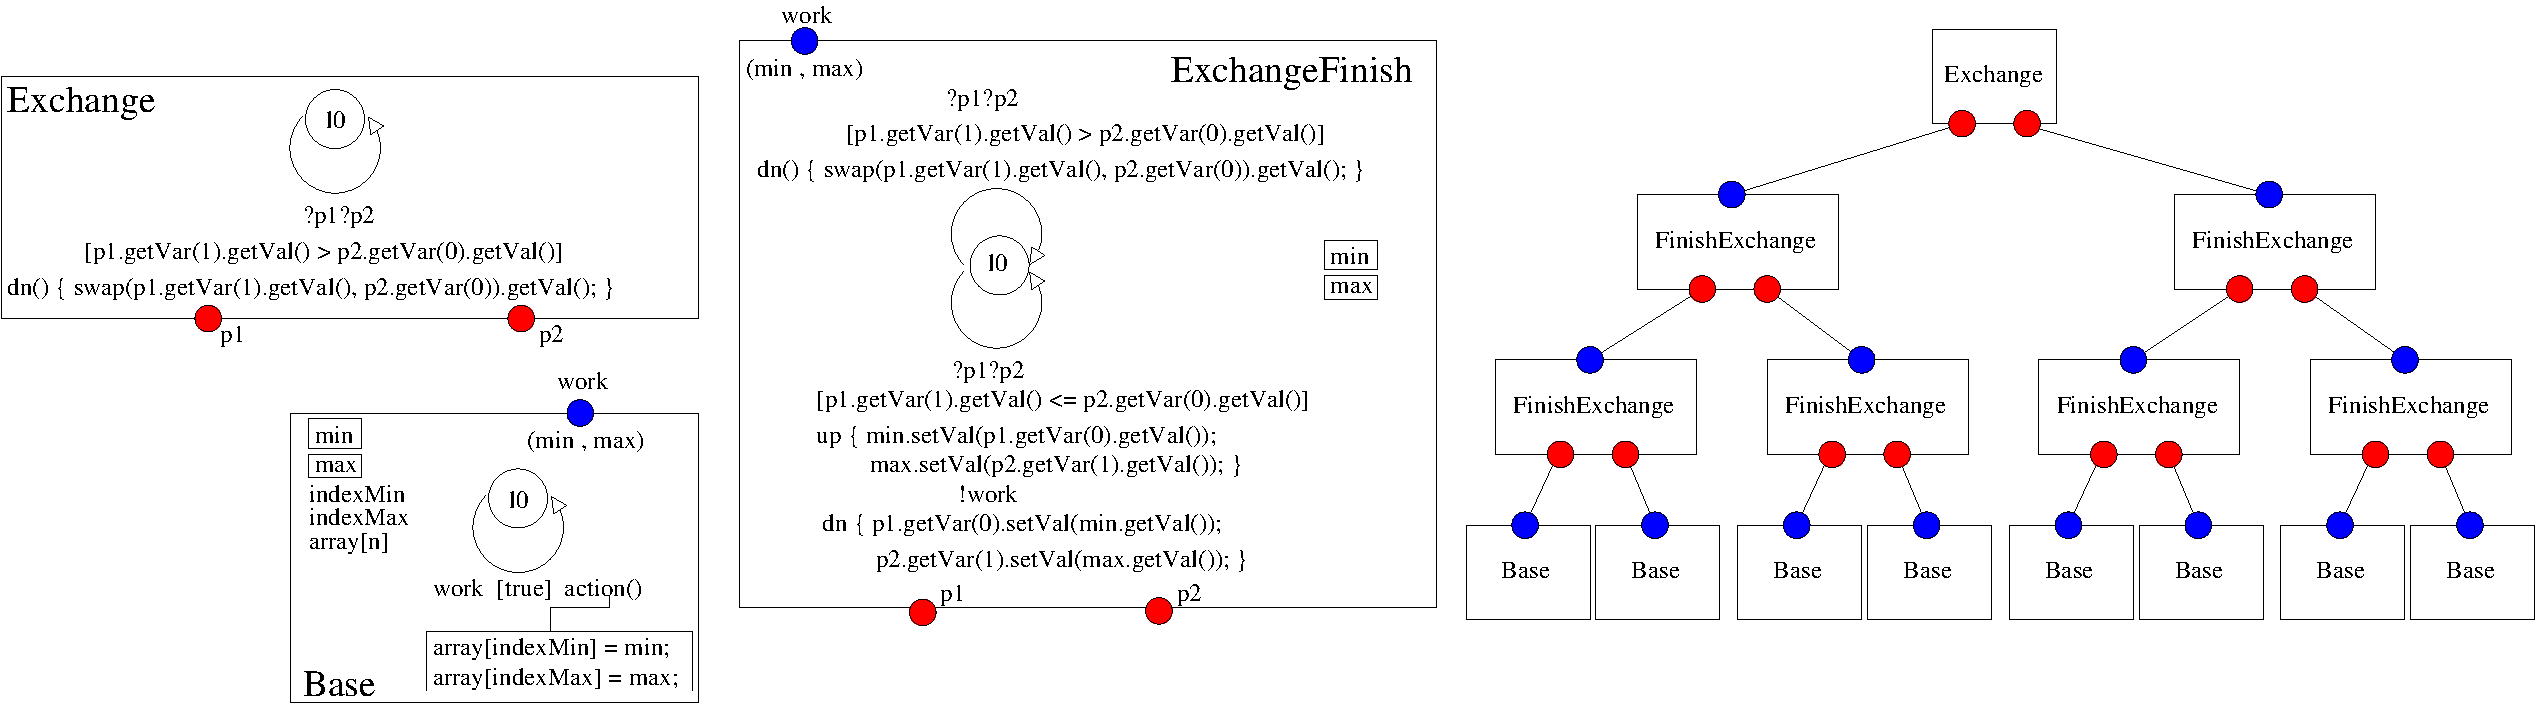
\includegraphics[scale=0.4]{fig/nsav2.pdf}
\caption{Network Sorting Algorithm in {\compmodel} - Merged Exchange and Finish Conversations}\label{fig:nsa2}
\end{figure}


Figure \ref{bench:nsa} shows the performance of NSA by considering different scenarios. As NSA model requires deterministic conversation components, we have ran this model with the two implementations (deterministic and non-deterministic). Figure \ref{bench:nsa1} shows that the non-deterministic implementation introduces a negligible overhead. Also we have compared the effect of merging conversation components which might improve the performance. 
We also study the efficiency of selecting all non-conflicting top conversation components before versus selecting only one top conversation component. Figure \ref{bench:nsa2} shows that selecting all non-conflicting top conversation components improve slightly the performance. 



\begin{figure} \centering
    \begin{subfigure}[b]{0.45\linewidth}
        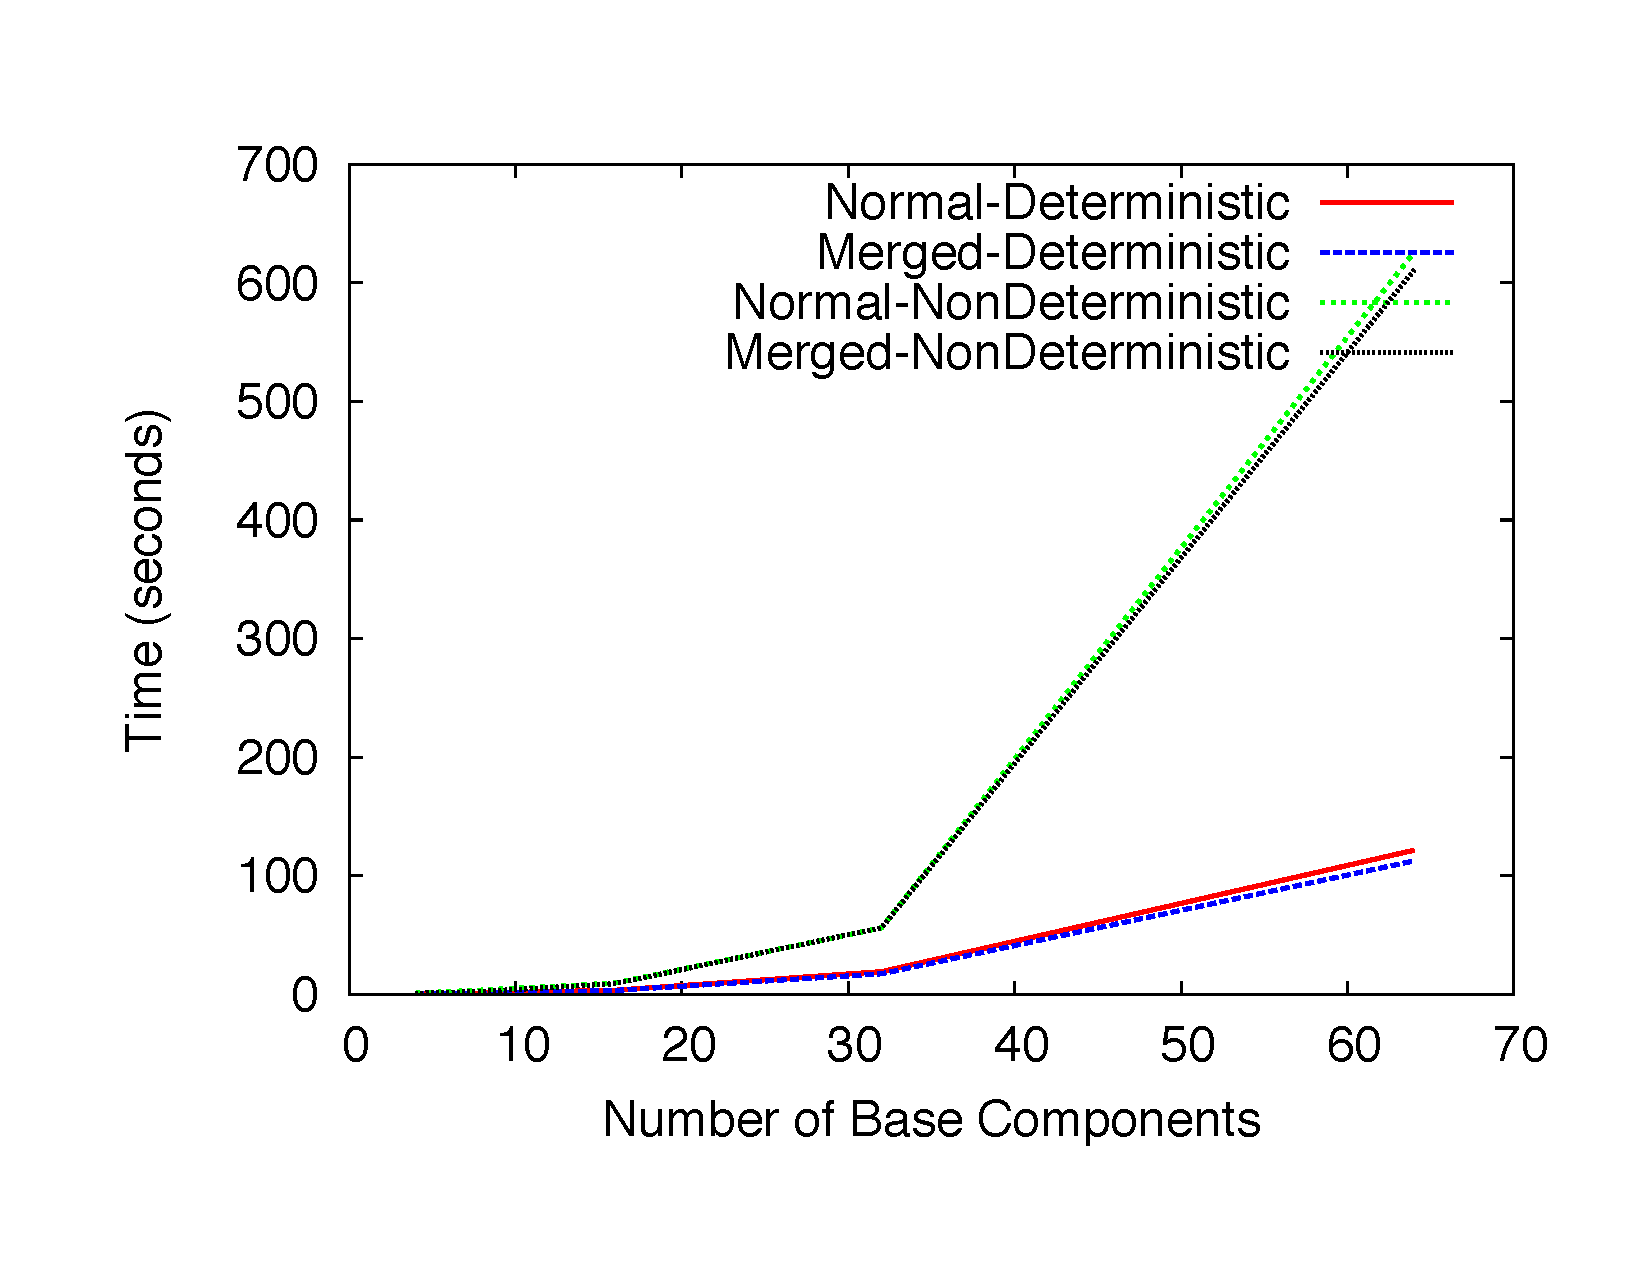
\includegraphics[scale=0.3]{bench/benchnsa1.pdf}
        \caption{Deterministic vs. Non-Deterministic}\label{bench:nsa1}
    \end{subfigure} %
    \quad
    \begin{subfigure}[b]{0.45\linewidth}    
        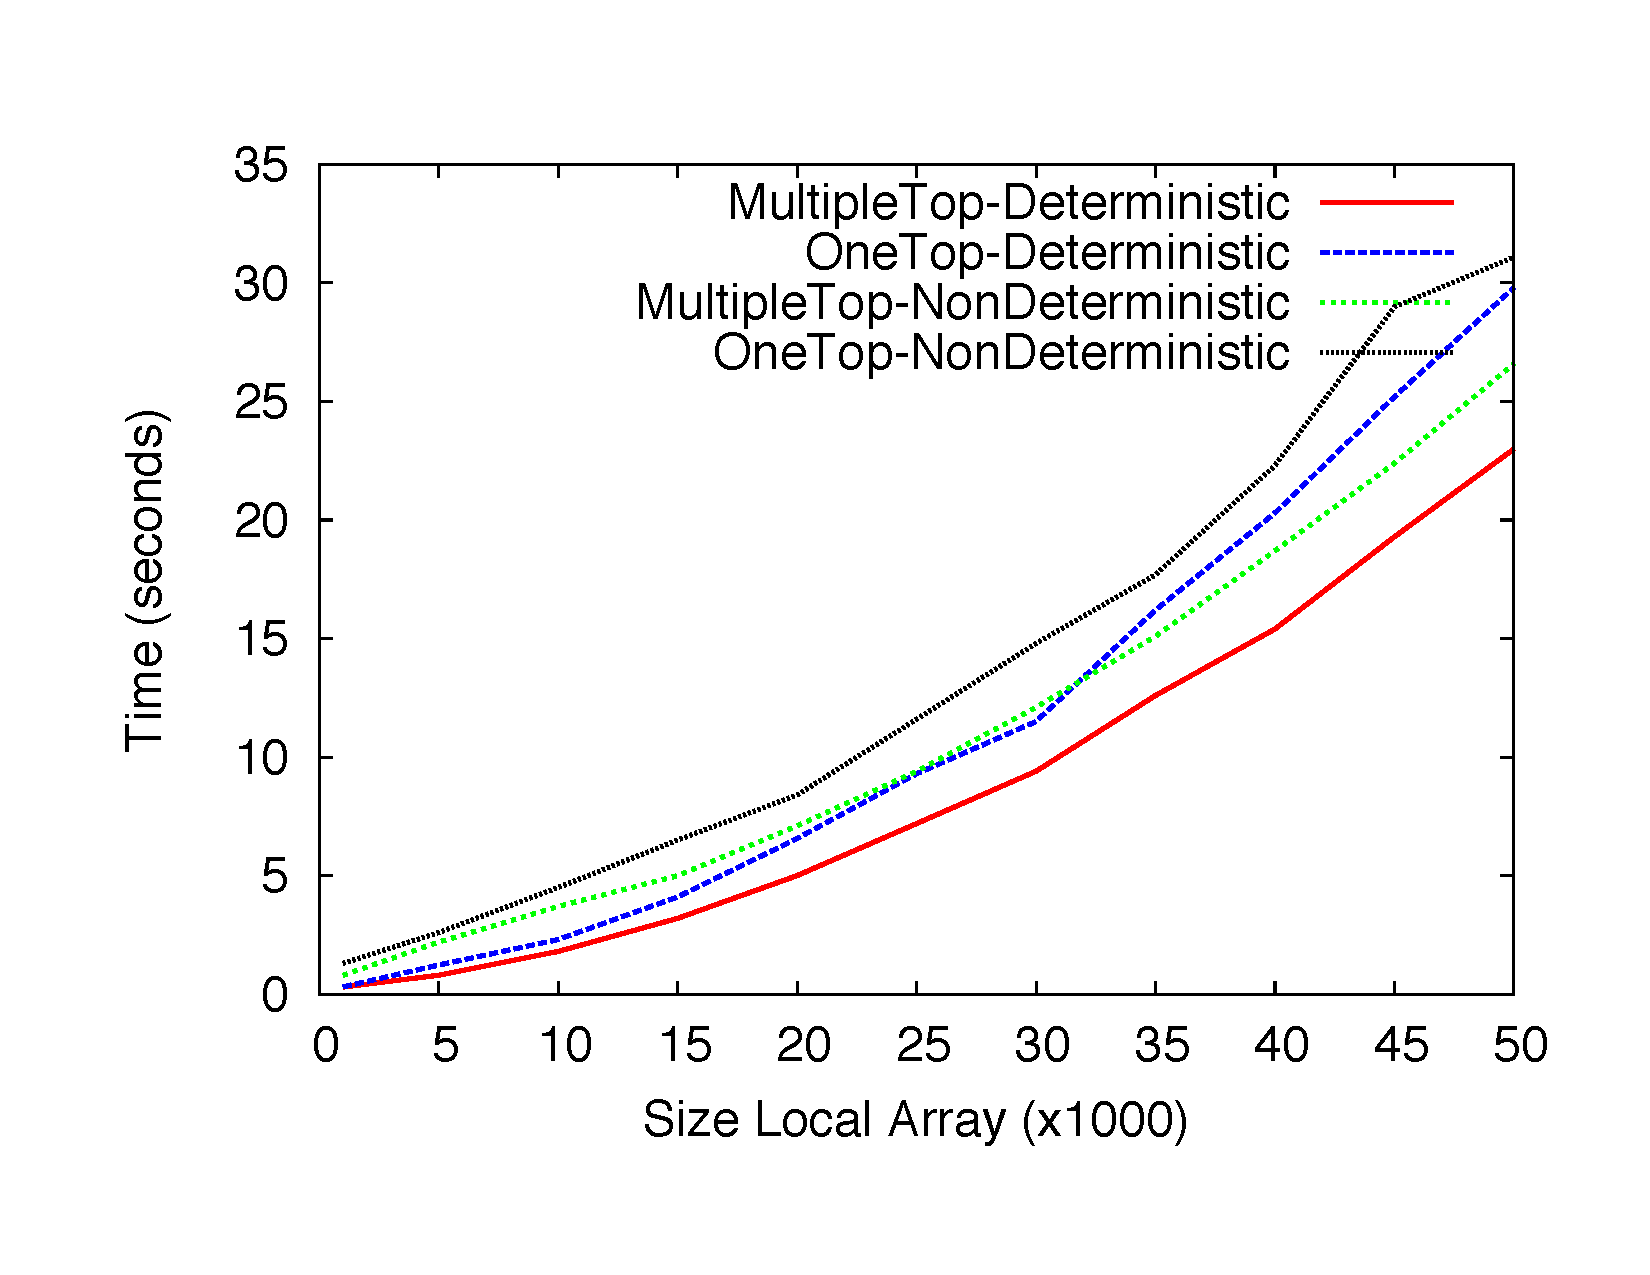
\includegraphics[scale=0.3]{bench/benchnsa2.pdf}
         \caption{One Top vs. Multiple-Top}\label{bench:nsa2}    
    \end{subfigure} 
    \caption{Performance (execution time in seconds) of NSA.}
    \label{bench:nsa}
\end{figure}

\subsection{Case Study: POTS}
\label{sec:pots}
We consider Plain Old Telephone Service (POTS), which provides voice connections between pairs of clients. Figure \ref{fig:pots} shows POTS in {\compmodel} model. 

\begin{figure} \centering
        \scalebox{0.5}{\input{fig/pots.pdf_t}}
        \caption{POTS in {\compmodel} model}\label{fig:pots}
\end{figure}

Figure \ref{bench:pots} shows the performance of POTS by varying the number of call to be satisfied.  

\begin{figure} 
\centering
        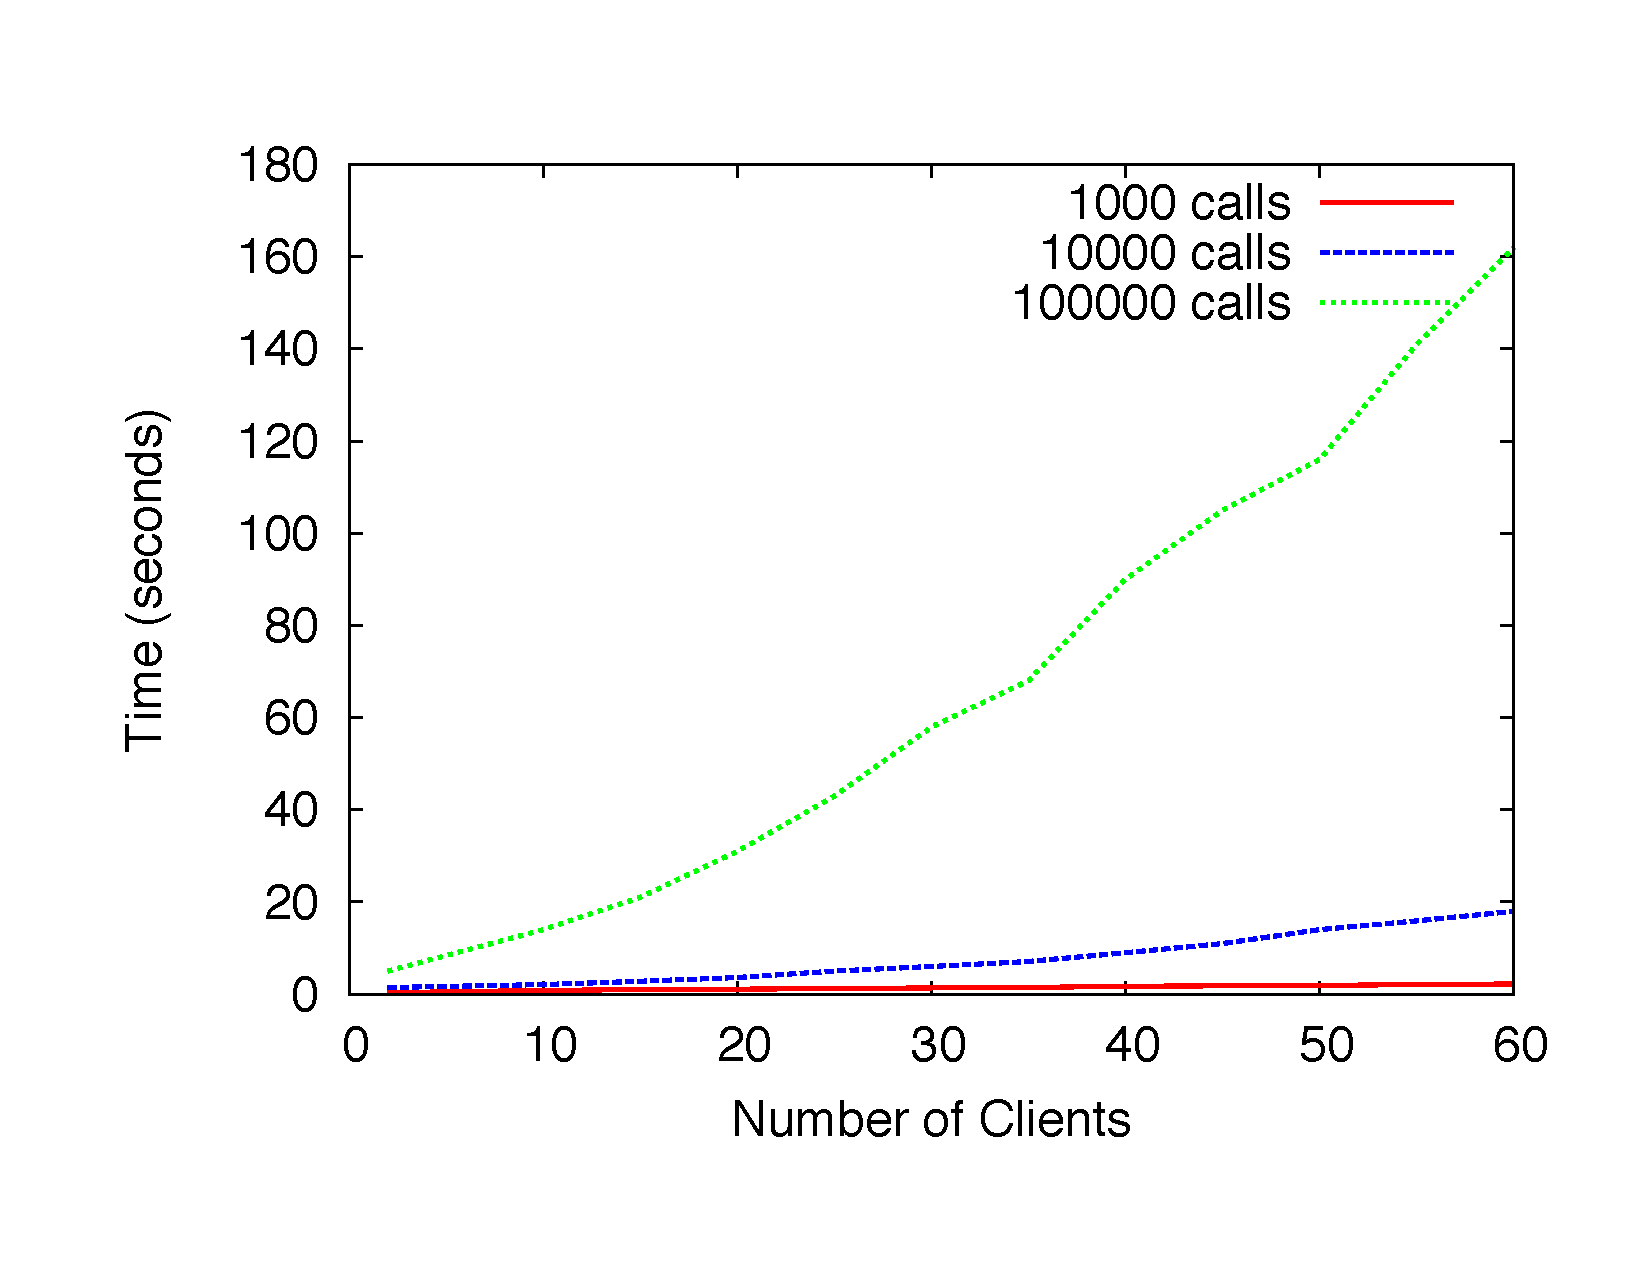
\includegraphics[scale=0.4]{bench/benchpots.pdf}
            \caption{Performance (execution time in seconds) of POTS.}
\label{bench:pots}
\end{figure}



% *********************************************************************
% *********************************************************************

\section{Case Study: POTS}
\label{sec:pots}


% *********************************************************************
% *********************************************************************

\section{Related Work}
\label{sec:related}


% *********************************************************************
% *********************************************************************

\section{Conclusion and Future Work}
\label{sec:conclusion}



\bibliographystyle{plain}
\bibliography{bip}

\end{document}
